\clearpage
\begingroup
\setlength{\emergencystretch}{1.5em}
\section{BM-ECSW with LSPG: implementation and first results}
\label{sec:implementation}

\textit{Working notes, October 4, 2026.} This section records our implementation of the mode-dependent weights proposed by Sebastian Rodriguez in Section~2. The test problem is the two-dimensional inviscid Burgers benchmark used in our workbench~\cite{impl-barnett2023}. We use an affine POD trial space and least-squares Petrov--Galerkin (LSPG) equations. Here, ``linear'' refers to the trial space: \textbf{the Burgers equations remain nonlinear}.

With the same \textbf{96-mode basis}, \textbf{225 consecutive training pairs}, and relative training tolerance $10^{-5}$, classical ECSW selects \textbf{2492 cells} and BM-ECSW \textbf{selects 300}. Both give trajectory errors close to $1\%$ against the high-dimensional model at three unseen parameter values. Three online runs per parameter give mean time ratios of \textbf{$5.45$--$7.17$} in favor of the current BM implementation. The following subsections define the equations, describe the algorithms, and document these measurements.

\paragraph{Notation.}
We follow the proposal's convention: \textbf{vectors} are bold with one underline, such as $\vect{y}$ and $\vect{R}$; \textbf{matrices} are bold with two underlines, such as $\matr{V}$ and $\matr{J}$. Individual entries, such as $y_i$, $K_{ij}$, and $\xi_{e,i}$, are scalars and have no underline.

\subsection{The Burgers problem and its discrete residual}
\label{sec:impl-burgers}

The state has two velocity components, $u_x(x_1,x_2,t)$ and $u_y(x_1,x_2,t)$. They evolve according to
\begin{equation}
 \frac{\partial \vect{U}}{\partial t}
 +\frac{\partial \vect{F}(\vect{U})}{\partial x_1}
 +\frac{\partial \vect{G}(\vect{U})}{\partial x_2}=\vect{S}(x_1;\vect{\mu}),
 \qquad \vect{U}=\begin{pmatrix}u_x\\u_y\end{pmatrix},
 \label{eq:impl-pde}
\end{equation}
where
\begin{equation}
 \vect{F}(\vect{U})=\begin{pmatrix}u_x^2/2\\u_xu_y/2\end{pmatrix},\qquad
 \vect{G}(\vect{U})=\begin{pmatrix}u_xu_y/2\\u_y^2/2\end{pmatrix},\qquad
 \vect{S}(x_1;\vect{\mu})=\begin{pmatrix}0.02\exp(\mu_2x_1)\\0\end{pmatrix}.
 \label{eq:impl-fluxes}
\end{equation}
The spatial domain is $[0,100]^2$, the final time is $25$, and the parameter domain is
\begin{equation}
 \vect{\mu}=(\mu_1,\mu_2)\in[4.25,5.50]\times[0.015,0.030].
\end{equation}
Initially, both velocity components are one. The parameter $\mu_1$ sets the incoming flux at the left boundary, while $\mu_2$ controls the source. In the discrete implementation, the prescribed incoming fluxes are $\vect{F}_{\mathrm{left}}=(\mu_1^2/2,0)^T$ and $\vect{G}_{\mathrm{bottom}}=(0,0)^T$. The top and right outgoing fluxes use the adjacent cell states.

The mesh contains $250\times250=62500$ cells. Each cell stores two velocity components, so the high-dimensional state $\vect{w}(t;\vect{\mu})$ has $N=125000$ entries. First-order upwind finite-volume flux differences give the semidiscrete system
\begin{equation}
 \dot{\vect{w}}+\mathcal L(\vect{w};\vect{\mu})=0.
 \label{eq:impl-hdm}
\end{equation}
The operator $\mathcal L$ includes flux differences, boundary contributions, and the negative of the source. Trapezoidal time integration with $\Delta t=0.05$ gives 500 steps. At step $n$, its residual is
\begin{equation}
 \vect{R}(\vect{w};\vect{w}^{n-1},\vect{\mu})=\vect{w}-\vect{w}^{n-1}
 +\frac{\Delta t}{2}\big[\mathcal L(\vect{w};\vect{\mu})+\mathcal L(\vect{w}^{n-1};\vect{\mu})\big].
 \label{eq:impl-residual}
\end{equation}
The high-dimensional model (HDM) solves $\vect{R}(\vect{w}^n;\vect{w}^{n-1},\vect{\mu})=0$. Its Jacobian with respect to the current state is
\begin{equation}
 \matr{J}(\vect{w};\vect{\mu})=\matr{I}+\frac{\Delta t}{2}\frac{\partial\mathcal L}{\partial \vect{w}}(\vect{w};\vect{\mu}).
 \label{eq:impl-jacobian}
\end{equation}

\begin{figure}[H]
 \centering
 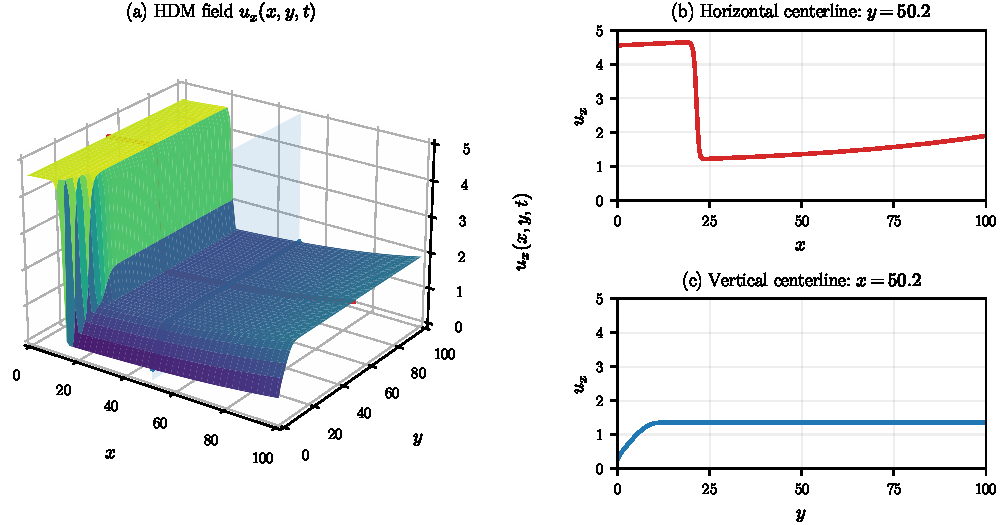
\includegraphics[width=0.96\linewidth]{figures/burgers_problem_3d.pdf}
 \caption{HDM Burgers solution at $\vect{\mu}=(4.56,0.019)$ and $t=7.5$: the $u_x$ field and two centerline cuts. This figure is reused from the Euclidean manuscript in \texttt{Project\_YvonMaday}.}
 \label{fig:impl-burgers}
\end{figure}

\subsection{From the POD coordinates to the LSPG equations}
\label{sec:impl-lspg}

The training parameters form the Cartesian product
\begin{equation}
 \{4.25,4.875,5.50\}\times\{0.015,0.0225,0.030\}.
\end{equation}
The nine HDM trajectories each contain 501 states, including the initial state. The POD snapshot matrix therefore has 4509 columns. We use the existing mean reference state $\vect{w}_{\mathrm{ref}}$ and $m=96$ orthonormal POD vectors, which retain $99.950267\%$ of the centered snapshot energy.

The affine approximation is
\begin{equation}
 \widehat{\vect{w}}(\vect{y})=\vect{w}_{\mathrm{ref}}+\matr{V}\vect{y},\qquad
 \matr{V}\in\mathbb R^{N\times m},\quad \vect{y}\in\mathbb R^m.
 \label{eq:impl-trial}
\end{equation}
The columns of $\matr{V}$ are the \textbf{modes}. The entries of $\vect{y}$ are their \textbf{amplitudes, or reduced coordinates}; they are not themselves modes. For example, with two columns, $\vect{y}=(1,2)^T$ means $\widehat{\vect{w}}=\vect{w}_{\mathrm{ref}}+\vect{v}_1+2\vect{v}_2$.

At each time step, the full projection-based reduced model (PROM) seeks to minimize
\begin{equation}
 \Phi(\vect{y})=\frac12\|\vect{R}(\widehat{\vect{w}}(\vect{y});\widehat{\vect{w}}^{n-1},\vect{\mu})\|_2^2.
 \label{eq:impl-lspg-objective}
\end{equation}
Write $\matr{A}(\vect{y})=\matr{J}(\widehat{\vect{w}}(\vect{y}))\matr{V}$. Applying the chain rule gives the LSPG stationarity equations~\cite{impl-carlberg2011}
\begin{equation}
 \vect{q}(\vect{y})=\nabla_y\Phi(\vect{y})=\matr{A}(\vect{y})^T \vect{R}(\widehat{\vect{w}}(\vect{y}))=0.
 \label{eq:impl-q}
\end{equation}
Thus the test matrix is $\matr{J}\matr{V}$, which changes with the current state. In this LSPG implementation, the quantity to approximate is $(\matr{J}\matr{V})^T\vect{R}$. This is the counterpart of $\matr{V}^T\vect{R}$ in the original proposal.

To identify the contribution of one cell $e$, take its two residual entries and the corresponding two rows of $\matr{A}$:
\begin{equation}
 \vect{r}_e=\begin{pmatrix}R_{u,e}\\R_{v,e}\end{pmatrix}\in\mathbb R^2,
 \qquad \matr{A}_e\in\mathbb R^{2\times m},
 \qquad \vect{c}_e=\matr{A}_e^T\vect{r}_e\in\mathbb R^m.
 \label{eq:impl-cell}
\end{equation}
For coordinate $i$, this means
\begin{equation}
 c_{e,i}=A_{u,e,i}R_{u,e}+A_{v,e,i}R_{v,e},\qquad
 \vect{q}=\sum_{e=1}^{62500}\vect{c}_e.
 \label{eq:impl-cell-component}
\end{equation}
Even though $\vect{q}$ has only 96 entries, evaluating this full sum still visits all 62500 cells. Hyper-reduction replaces that sum by a weighted sum over a smaller set, following the mesh-sampling approach for Petrov--Galerkin models~\cite{impl-grimberg2021}.

\subsection{What classical and by-mode weights change}
\label{sec:impl-weights}

Let $\widetilde E$ denote the selected cells. Classical ECSW assigns one nonnegative scalar $\xi_e$ to each selected cell:
\begin{equation}
 \widetilde{\vect{q}}^{\mathrm{ECSW}}(\vect{y})
 =\sum_{e\in\widetilde E}\xi_e \matr{A}_e(\vect{y})^T\vect{r}_e(\vect{y}).
 \label{eq:impl-classical}
\end{equation}
\textbf{The same weight multiplies all 96 components} of that cell's contribution. These equations are the gradient of the sampled objective
\begin{equation}
 \Phi_{\mathrm{ECSW}}(\vect{y})
 =\frac12\sum_{e\in\widetilde E}\xi_e\|\vect{r}_e(\vect{y})\|_2^2.
 \label{eq:impl-classical-objective}
\end{equation}
For a Gauss--Newton step, we stack the blocks
\begin{equation}
 \vect{r}_\xi=\begin{bmatrix}\sqrt{\xi_{e_1}}\vect{r}_{e_1}\\\vdots\\\sqrt{\xi_{e_s}}\vect{r}_{e_s}\end{bmatrix},
 \qquad
 \matr{A}_\xi=\begin{bmatrix}\sqrt{\xi_{e_1}}A_{e_1}\\\vdots\\\sqrt{\xi_{e_s}}A_{e_s}\end{bmatrix}
\end{equation}
and solve $\min_p\|\matr{A}_\xi \vect{p}+\vect{r}_\xi\|_2$. The square root is essential: the product $\matr{A}_\xi^T\vect{r}_\xi$ then contains $\xi_e$, as required by Equation~\eqref{eq:impl-classical}. Multiplying both blocks by $\xi_e$ would instead give $\xi_e^2$.

BM-ECSW assigns a weight $\xi_{e,i}\geq0$ to each cell--coordinate pair:
\begin{equation}
 \widetilde q_i^{\mathrm{BM}}(\vect{y})
 =\sum_{e\in\widetilde E}\xi_{e,i}c_{e,i}(\vect{y}),
 \qquad i=1,\ldots,m.
 \label{eq:impl-bm}
\end{equation}
There is \textbf{one shared cell set}, but its \textbf{weights may differ between coordinates}. A selected cell may have zero weight for some coordinates. The classical rule is contained in this family: setting $\xi_{e,i}=\xi_e$ for every $i$ recovers Equation~\eqref{eq:impl-classical}.

For each coordinate separately, $\widetilde q_i^{\mathrm{BM}}=\partial\Phi_i/\partial y_i$, where
\begin{equation}
 \Phi_i(\vect{y})=\frac12\sum_{e\in\widetilde E}\xi_{e,i}\|\vect{r}_e(\vect{y})\|_2^2.
\end{equation}
However, the assembled vector need not be the gradient of a single scalar function. The mixed derivatives can differ. Consequently, a single square-root-weighted residual and its usual Gauss--Newton step do not implement general mode-dependent weights. We solve Equation~\eqref{eq:impl-bm} directly with Newton's method.

Here $\Phi$ is a residual least-squares objective, not a mechanical potential energy. The structural energy argument in reading note~4 motivates a question about what is preserved; it does not by itself establish energy conservation or its loss for this forced Burgers problem with inflow boundaries.

\subsection{Offline training: states, matrices, and selection}
\label{sec:impl-training}

\paragraph{Which states are used?}
For each HDM snapshot, we first project onto the affine trial space:
\begin{equation}
 \overline{\vect{w}}^{\,n}
 =\vect{w}_{\mathrm{ref}}+\matr{V}\matr{V}^T(\vect{w}_{\mathrm{HDM}}^n-\vect{w}_{\mathrm{ref}}).
 \label{eq:impl-projection}
\end{equation}
A training pair consists of projected current and previous states. For the matched comparison, they are consecutive: $(\overline{\vect{w}}^{\,n},\overline{\vect{w}}^{\,n-1})$. The training residual is evaluated on this pair using Equation~\eqref{eq:impl-residual}, and $\matr{J}\matr{V}$ is evaluated at its current state. These projected HDM pairs generally have nonzero residuals, even though the unprojected HDM trajectory solves the full equations.

The global parameter--time stratified sampler uses seed 42 and selects 25 pairs from each of the nine training parameters, giving $n_s=225$ pairs. The explicit count is fixed before training; the number of sampled cells is determined by the tolerance. In this implementation the admissible current indices run from the offset to 499, so the state at index 500 is not a training current state.

An additional experiment uses offset 3: its pair is $(\overline{\vect{w}}^{\,n},\overline{\vect{w}}^{\,n-3})$. The residual still uses $\Delta t=0.05$; this is an altered training pair, not a three-step time integrator. Online simulation always uses $n-1$. Offset 3 changes both the previous state and the sampler's admissible indices, so this experiment does not share exactly the same training data as offset 1.

\paragraph{How is the matrix assembled?}
For pair $j$, calculate all $\vect{c}_e^{(j)}$ from Equation~\eqref{eq:impl-cell}. The matrix named $\matr{C}$ in the implementation is the stacked contribution matrix $\matr{G}$ of the proposal:
\begin{equation}
 C_{(j-1)m+i,e}=c_{e,i}^{(j)},\qquad
 \matr{C}\in\mathbb R^{n_sm\times62500},\qquad \vect{b}=\matr{C}\vect{1}.
 \label{eq:impl-C}
\end{equation}
Each column is one candidate cell. Each row corresponds to one training pair and one coordinate. With 225 pairs and 96 modes, $\matr{C}$ has $21600\times62500$ entries. No SVD compression of this contribution matrix is used in these ECSW experiments.

For BM, take the rows belonging to coordinate $i$:
\begin{equation}
 G^{[i]}_{j,e}=c_{e,i}^{(j)},\qquad
 \matr{G}^{[i]}\in\mathbb R^{225\times62500},\qquad
 \vect{b}^{[i]}=\matr{G}^{[i]}\vect{1}.
 \label{eq:impl-Gi}
\end{equation}
The 96 matrices $\matr{G}^{[i]}$ partition the rows of $\matr{C}$; their total number of entries is unchanged. BM gains flexibility through separate weight vectors, not by creating more training entries.

\paragraph{What is fitted after selecting a cell?}
On a current cell set $\widetilde E$, classical ECSW solves
\begin{equation}
 \vect{\xi}^*=\underset{\vect{z}\geq0}{\arg\min}\;
 \|\matr{C}(:,\widetilde E)\vect{z}-\vect{b}\|_2^2.
 \label{eq:impl-classical-nnls}
\end{equation}
BM solves one nonnegative least-squares (NNLS) problem per coordinate:
\begin{equation}
 \vect{\xi}_i^*=\underset{\vect{z}\geq0}{\arg\min}\;
 \|\matr{G}^{[i]}(:,\widetilde E)\vect{z}-\vect{b}^{[i]}\|_2^2.
 \label{eq:impl-bm-nnls}
\end{equation}
These are \textbf{final weights on the selected set}: every selected weight can be readjusted. \textbf{The right-hand side is the original target} $\vect{b}$ or $\vect{b}^{[i]}$. The current residual is used for scoring candidates, not substituted for that target in a final-weight NNLS solve. This is the distinction discussed in reading note~3.

\begin{algorithm}[H]
 \caption{BM-ECSW training with a shared cell set}
 \label{alg:impl-offline}
 \small
 \begin{algorithmic}[1]
  \Require $\matr{G}^{[i]}$, $\vect{b}^{[i]}$, $i=1,\ldots,m$; relative tolerance $\varepsilon=10^{-5}$
  \Ensure Shared cells $\widetilde E$ and nonnegative weights $\xi_{e,i}$
  \State $\widetilde E\gets\varnothing$; $\vect{h}^{[i]}\gets \vect{b}^{[i]}$ for all $i$
  \State $\beta\gets\sum_i\|\vect{b}^{[i]}\|_2^2$
  \While{$\sqrt{\sum_i\|\vect{h}^{[i]}\|_2^2/\beta}>\varepsilon$}
   \State $\vect{\mu}\gets\sum_i (\matr{G}^{[i]})^T \vect{h}^{[i]}$
   \State Consider only cells outside $\widetilde E$; select $e^*\gets\arg\max_e\mu_e$
   \If{no positive candidate score remains}
    \State Stop and report that the requested tolerance was not attained
   \EndIf
   \State $\widetilde E\gets\widetilde E\cup\{e^*\}$
   \For{$i=1,\ldots,m$}
    \State $\vect{\xi}_i\gets\arg\min_{z\geq0}\|\matr{G}^{[i]}(:,\widetilde E)\vect{z}-\vect{b}^{[i]}\|_2^2$
    \State $\vect{h}^{[i]}\gets \vect{b}^{[i]}-\matr{G}^{[i]}(:,\widetilde E)\vect{\xi}_i$
   \EndFor
  \EndWhile
  \State Discard any cell whose weights are zero for every coordinate
 \end{algorithmic}
\end{algorithm}

The signed score follows the proposal. Contributions from different coordinates can cancel in this score; the implementation does not replace it by a sum of absolute values or predicted decreases. \textbf{The stopping criterion is global}:
\begin{equation}
 \eta=\sqrt{\frac{\sum_i\|\vect{h}^{[i]}\|_2^2}{\sum_i\|\vect{b}^{[i]}\|_2^2}}
 \leq10^{-5}.
 \label{eq:impl-tolerance}
\end{equation}
It does not impose $10^{-5}$ separately on every coordinate. The code option \texttt{ecsw\_tol\_squared} is $10^{-10}$, since it compares the squared ratio. Classical ECSW uses the same global relative tolerance for $\|\matr{C}\vect{\xi}-\vect{b}\|_2/\|\vect{b}\|_2$. Its QR updates accelerate the selected-column NNLS calculations, and its final fit is checked against the original contribution matrix.

\subsection{Online evaluation and the exact BM Jacobian}
\label{sec:impl-online}

\paragraph{Weighted cells and support cells.}
A residual at cell $e$ needs its own state and its upstream neighbors in the $x_1$ and $x_2$ directions. The augmented mesh contains the weighted cells and these support cells. We reconstruct $\vect{w}_{\mathrm{ref}}+\matr{V}\vect{y}$ only on this augmented mesh during time stepping. Support cells provide the stencil states; they add no term to the ECSW sum unless they are also weighted cells.

For the matched rules, classical ECSW uses 2492 weighted cells and 5914 augmented cells. BM uses 300 weighted cells and 868 augmented cells. The BM state reconstruction therefore has 1736 entries, while its sampled residual has 600 entries. Both methods still solve for 96 reduced coordinates.

\paragraph{Differentiating the BM equations.}
For fixed previous state, define $H_{e,\alpha,ij}=\partial^2R_{e,\alpha}/(\partial y_i\partial y_j)$, where $\alpha$ denotes one of the two velocity components. Since $A_{e,\alpha,i}=\partial R_{e,\alpha}/\partial y_i$, differentiation gives
\begin{equation}
 K_{ij}=\frac{\partial\widetilde q_i^{\mathrm{BM}}}{\partial y_j}
 =\sum_{e\in\widetilde E}\xi_{e,i}
 \left[\sum_{\alpha=1}^2 A_{e,\alpha,i}A_{e,\alpha,j}
       +\sum_{\alpha=1}^2R_{e,\alpha}H_{e,\alpha,ij}\right].
 \label{eq:impl-K}
\end{equation}
The \textbf{weight carries index $i$}, the equation being differentiated, even when the derivative is with respect to $y_j$. Using the weights of coordinate $j$ would give a different matrix. Generally $K_{ij}\ne K_{ji}$.

Writing $\Xi_{e,i}=\xi_{e,i}$ and collecting the two component rows as $\matr{A}_u,\matr{A}_v$, the first term is evaluated with vectorized products:
\begin{equation}
 \matr{K}_{\mathrm{first}}=(\matr{\Xi}\odot \matr{A}_u)^T\matr{A}_u+(\matr{\Xi}\odot \matr{A}_v)^T\matr{A}_v,
\end{equation}
where $\odot$ is entrywise multiplication. \textbf{The residual Hessian term is also retained}. Burgers' quadratic fluxes make these second derivatives available analytically. This is the exact derivative of the BM equations, rather than a Gauss--Newton approximation.

Finite-difference checks at an actual first-step state gave relative Jacobian errors below $8\times10^{-11}$ with coordinate perturbations of $10^{-3}$. Regression checks also cover derivatives with respect to the previous reduced state and the limit of identical weights across coordinates. These checks preceded the runs reported below.

\begin{algorithm}[H]
 \caption{One BM-ECSW time step}
 \label{alg:impl-online}
 \small
 \begin{algorithmic}[1]
  \Require Previous coordinates $\vect{y}^{n-1}$; sampled weights, basis, and stencil operators
  \Ensure Current coordinates $\vect{y}^n$ and the nonlinear solver status
  \State $\vect{y}\gets \vect{y}^{n-1}$; evaluate $\widetilde{\vect{q}}(\vect{y})$ and $\matr{K}(\vect{y})$
  \State $q_0\gets\|\widetilde{\vect{q}}(\vect{y})\|_2$ (use 1 if this norm is zero)
  \For{at most 20 nonlinear iterations}
   \If{$\|\widetilde{\vect{q}}(\vect{y})\|_2/q_0<10^{-5}$}
    \State Return $\vect{y}$ with status converged
   \EndIf
   \State Solve $\matr{K}\vect{p}=-\widetilde{\vect{q}}$; use a least-squares solve if $\matr{K}$ is singular
   \State Try $\vect{y}+\alpha \vect{p}$, starting with $\alpha=1$ and halving up to 24 trials
   \State Accept a trial if $\|\widetilde{\vect{q}}(\vect{y}+\alpha \vect{p})\|_2<(1-10^{-12})\|\widetilde{\vect{q}}(\vect{y})\|_2$
   \If{the Newton direction has no accepted trial}
    \State Try the same backtracking with a scaled direction $-\matr{K}^T\widetilde{\vect{q}}$
   \EndIf
   \If{neither direction is accepted, or the step is nonfinite}
    \State Stop and report the failure reason
   \EndIf
   \State Update $\vect{y}$ and reevaluate $\widetilde{\vect{q}},\matr{K}$
  \EndFor
  \State Check the final tolerance and return the coordinates and status
 \end{algorithmic}
\end{algorithm}

The fallback direction decreases the merit function $\|\widetilde{\vect{q}}\|_2^2/2$ locally when its gradient is nonzero. Its length is set to $\min(\max(\|\vect{p}\|_2,1),100)$. This merit function helps find a root; it is not the original LSPG residual objective.

The classical implementation uses square-root-weighted Gauss--Newton with a least-squares linear solve. It can stop when the sampled residual has decreased by a relative factor $10^{-5}$, or when the relative change between successive residual norms is below $10^{-2}$. BM uses the projected-equation tolerance in Algorithm~\ref{alg:impl-online}. Both have a 20-iteration budget, but \textbf{their stopping quantities differ}. The timing comparison below therefore includes the effects of both the sampled rules and these solver choices.

\subsection{Numerical results}
\label{sec:impl-results}

\paragraph{Cells selected by the training tolerance.}
Table~\ref{tab:impl-cubature} uses 225 pairs in every row. The first two rows form the matched comparison: identical basis, consecutive-pair training policy, seed, and tolerance. The last row is the additional BM offset-3 experiment. All three rules meet the requested relative training tolerance. The counts are final cells with nonzero weights.

\begin{table}[H]
 \centering\small
 \begin{tabular}{@{}lrrrrl@{}}
\toprule
Rule & Offset & Cells & Augmented & Weight entries & Training error\\
\midrule
Classical ECSW & 1 & 2\,492 & 5\,914 & 2\,492 & $9.795\times10^{-6}$\\
BM-ECSW & 1 & 300 & 868 & 21\,597 & $8.359\times10^{-6}$\\
BM-ECSW & 3 & 276 & 813 & 21\,445 & $9.819\times10^{-6}$\\
\bottomrule
\end{tabular}

 \caption{Trained rules with 96 modes and 225 pairs. ``Augmented'' includes stencil support. ``Weight entries'' counts strictly positive scalar weights. Training error is the relative norm in Equation~\eqref{eq:impl-tolerance}.}
 \label{tab:impl-cubature}
\end{table}

BM with offset 1 has $8.31$ times fewer weighted cells and $6.81$ times fewer augmented cells than the matched classical rule. It stores more positive scalar weights: 21597 rather than 2492. This is a trade-off between weight storage and evaluating fewer residual stencils. The number of online unknowns remains 96. Offset 3 reduces the BM weighted-cell count by another $8\%$, from 300 to 276.

\begin{figure}[H]
 \centering
 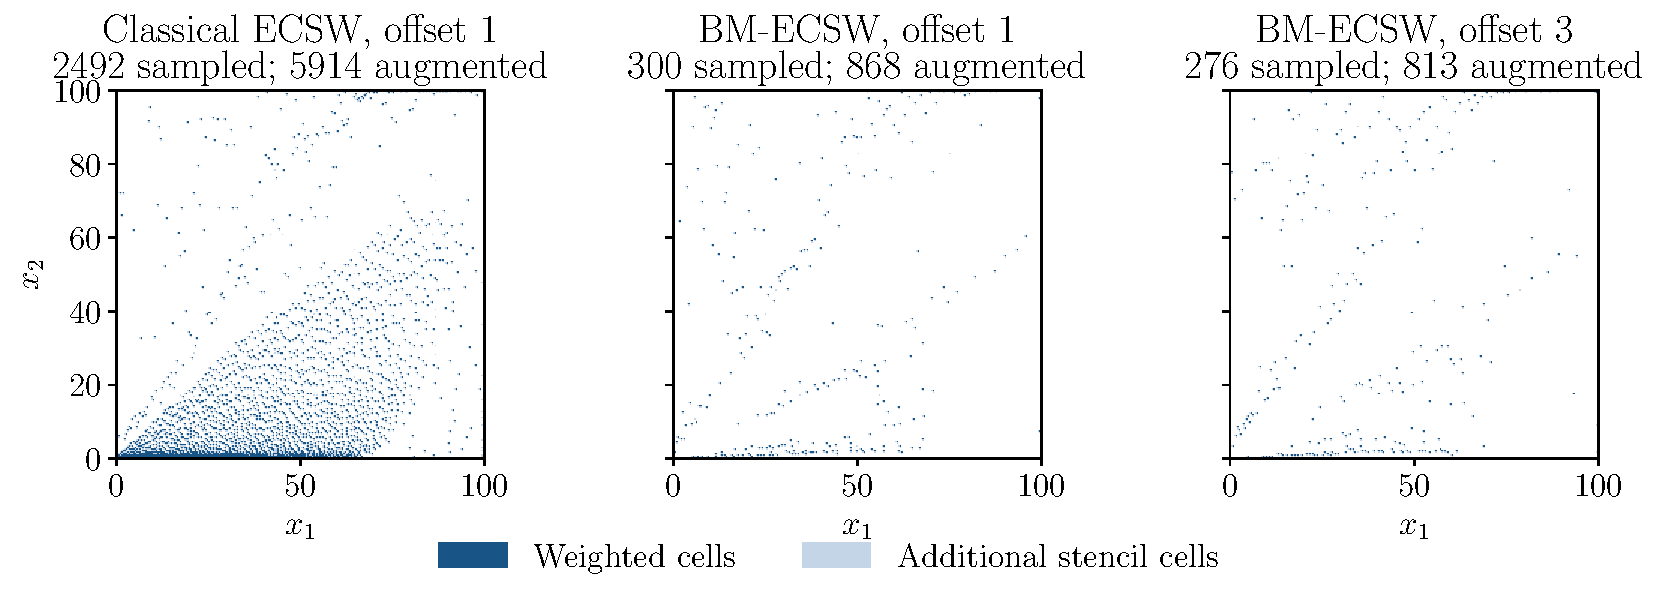
\includegraphics[width=\linewidth]{figures/sampled_cells.pdf}
 \caption{Weighted cells (dark blue) and additional stencil support (light blue). The classical and BM offset-1 rules use matched training. The BM offset-3 rule uses different training pairs.}
 \label{fig:impl-meshes}
\end{figure}

\paragraph{Errors against the HDM.}
We evaluate three parameter values inside the training parameter domain but outside its nine-point grid. Let $\matr{W}$ collect both velocity fields at all 501 times. The reported trajectory error is
\begin{equation}
 e_{\mathrm{HDM}}=100\frac{\|\matr{W}_{\mathrm{HPROM}}-\matr{W}_{\mathrm{HDM}}\|_F}{\|\matr{W}_{\mathrm{HDM}}\|_F}.
 \label{eq:impl-error}
\end{equation}
Here HPROM denotes the hyper-reduced projection-based model. This error includes both trial-space approximation and hyper-reduction effects; it is not a pure cubature error.

\begin{table}[H]
 \centering\small
 \begin{tabular}{@{}rrrrr@{}}
\toprule
$\mu_1$ & $\mu_2$ & Classical ECSW & BM, offset 1 & BM, offset 3\\
\midrule
4.56 & 0.019 & 1.0959 & 1.1019 & 1.1169\\
4.75 & 0.020 & 1.0011 & 1.0061 & 1.0209\\
5.19 & 0.026 & 0.9928 & 1.0069 & 1.0106\\
\bottomrule
\end{tabular}

 \caption{Full-trajectory errors in percent against the HDM. All rules have 225 training pairs.}
 \label{tab:impl-accuracy}
\end{table}

The two BM rules complete all \textbf{500 time steps at all three evaluation parameters} with the projected-equation tolerance satisfied within the 20-iteration budget. The offset-1 BM errors are slightly smaller than the offset-3 BM errors, though the latter uses fewer cells. We choose the 300-cell offset-1 rule for repeated timing because it has lower observed errors and matches the classical rule's training data.

\paragraph{Three repeated online runs.}
We run each method three times at each parameter, giving 18 runs. Each run starts a fresh Python process. Execution is sequential, with parameter and method order varied between repetitions, and uses 20 CPU threads on an Intel Core Ultra 7 265 processor. Actual numerical-library thread pools are recorded in each run's metadata. No additional warm-up run is discarded.

The timer covers the production HPROM function: mesh and operator setup, initial reduced projection, and 500 time steps. It excludes offline training, Python startup, loading the basis and weights, full-field reconstruction after integration, HDM error calculations, plotting, and output files. Setup still includes operations involving the full mesh; the sampled calculations described above concern time stepping.

\begin{table}[H]
 \centering\small
 \begin{tabular}{@{}llrrrrr@{}}
\toprule
Parameter & Computational model & Run 1 & Run 2 & Run 3 & Mean & SD\\
\midrule
$(4.56,0.019)$ & HPROM (ECSW) & 18.889 & 18.945 & 17.795 & 18.543 & 0.648\\
$(4.56,0.019)$ & HPROM (BM-ECSW) & 1.238 & 1.205 & 1.212 & 1.218 & 0.017\\
\addlinespace
$(4.75,0.020)$ & HPROM (ECSW) & 19.682 & 18.408 & 18.390 & 18.827 & 0.741\\
$(4.75,0.020)$ & HPROM (BM-ECSW) & 1.209 & 1.204 & 1.200 & 1.204 & 0.005\\
\addlinespace
$(5.19,0.026)$ & HPROM (ECSW) & 17.304 & 19.880 & 18.526 & 18.570 & 1.288\\
$(5.19,0.026)$ & HPROM (BM-ECSW) & 1.206 & 1.211 & 1.208 & 1.208 & 0.002\\
\addlinespace
\bottomrule
\end{tabular}

 \caption{Online times in seconds, with arithmetic mean and sample standard deviation (SD) over three runs. BM denotes the 300-cell offset-1 rule.}
 \label{tab:impl-timings}
\end{table}

\begin{table}[H]
 \centering\small
 \begin{tabular}{@{}rrrrr@{}}
\toprule
\textbf{$\mu_1$} & \textbf{$\mu_2$} & \textbf{ECSW mean [s]} & \textbf{BM mean [s]} & \textbf{Ratio}\\
\midrule
4.56 & 0.019 & 24.811 & 4.552 & $5.450\times$\\
4.75 & 0.020 & 22.425 & 3.486 & $6.433\times$\\
5.19 & 0.026 & 21.469 & 2.993 & $7.172\times$\\
\bottomrule
\end{tabular}

 \caption{Ratio of the mean classical ECSW time to the mean BM-ECSW time.}
 \label{tab:impl-speedups}
\end{table}

\begin{figure}[H]
 \centering
 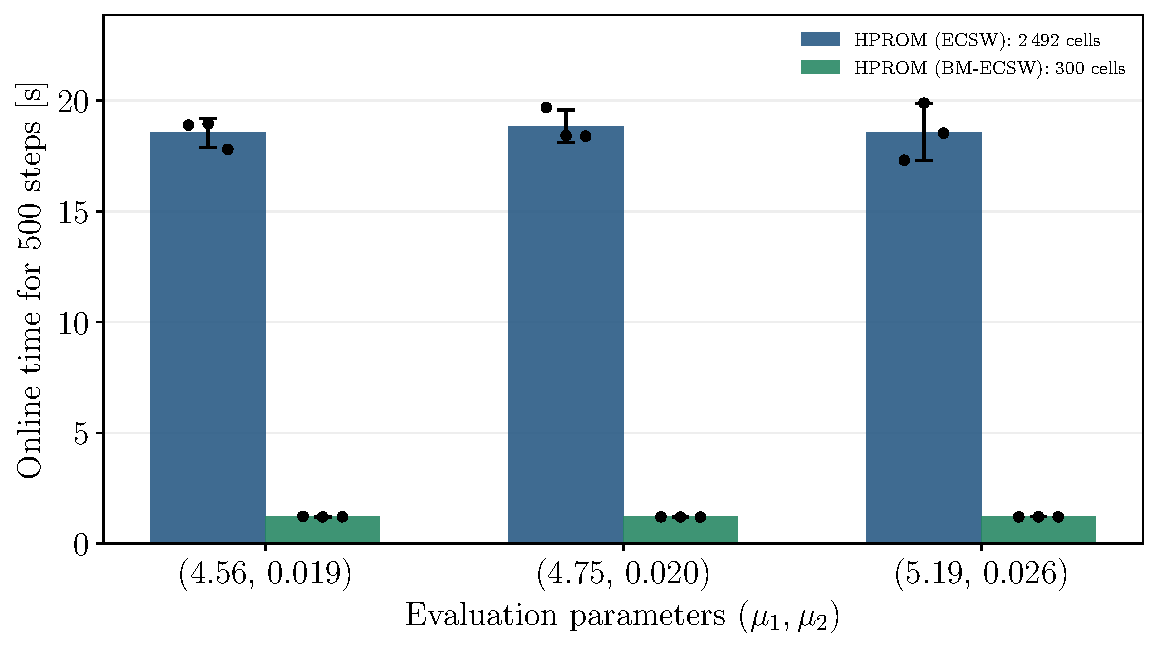
\includegraphics[width=0.90\linewidth]{figures/online_timings.pdf}
 \caption{Repeated online measurements. Bars show means, points show individual runs, and error bars show sample standard deviations.}
 \label{fig:impl-timings}
\end{figure}

The trajectory errors are unchanged across repetitions. The recorded nonlinear iteration counts are 1500 for classical ECSW and 1503 for BM per 500-step run, including convergence checks. BM satisfies its projected-equation tolerance on all 4500 time steps across the nine timed BM runs. Thus the measured speed difference does not arise from BM simply taking fewer nonlinear iterations. Fewer sampled and support cells reduce work, but solver algebra and stopping criteria also differ. Three repetitions document the variability observed on this machine; they do not establish a general speed ratio for other problems or implementations.

\subsection{Why fitting 90 pairs was not sufficient}
\label{sec:impl-diagnostic}

Earlier BM rules had excellent training fits but failed online. With 90 offset-3 pairs, 124 cells gave a relative training error of $6.42\times10^{-7}$; with 90 consecutive pairs, 145 cells gave $1.28\times10^{-15}$. After correcting and checking the Jacobian, these rules still satisfied the nonlinear tolerance at only 36 and 5 of the 500 steps, respectively, at $\vect{\mu}=(4.56,0.019)$. Their trajectory errors against the HDM were approximately $4483\%$ and $5357\%$. Increasing the training fit accuracy alone did not solve the problem.

To examine this, we compute a fresh full PROM trajectory and compare one-step solves using the same previous PROM state. The reference uses the production Gauss--Newton solver with its residual/plateau stopping criterion; it is not an exact stationarity solve. Fifteen time indices are probed, including early, intermediate, and late times. All tested BM rules can solve their own one-step equations within 20 iterations at these shared states. \textbf{Solving those equations is therefore different from obtaining a time update close to the full PROM update}.

Table~\ref{tab:impl-diagnostic} shows the first step. Its state errors are against the full PROM, not the HDM, and use both velocity fields. For these equation diagnostics, every rule, including the classical rule, uses Newton for its one-step root solve. The condition number is evaluated at the common initial predictor. The sensitivity norm is evaluated near each method's own root.

\begin{table}[H]
 \centering\small
 \begin{tabular}{@{}lrrrr@{}}
\toprule
Rule & Pairs & State error [\%] & $\kappa_2(\matr{K})$ & $\|\matr{T}\|_2$\\
\midrule
Classical, offset 3 & 90 & 0.000919 & 1.077 & 1.0032\\
BM, offset 3 & 90 & 2.706970 & 465.713 & 2.4886\\
BM, offset 1 & 90 & 30.626509 & 3\,280.493 & 7.0456\\
BM, offset 1 & 225 & 0.048015 & 13.403 & 1.0036\\
\bottomrule
\end{tabular}

 \caption{First-step diagnostic at $\vect{\mu}=(4.56,0.019)$ using a shared previous PROM state. $\matr{K}$ is the derivative of the reduced equations; $\matr{T}$ is the local derivative of the implicit time update. The classical row uses the earlier 90-pair rule, not the 2492-cell benchmark rule.}
 \label{tab:impl-diagnostic}
\end{table}

To define the sensitivity, write the step equations as $\widetilde{\vect{q}}(\vect{y}^n,\vect{y}^{n-1})=0$ and set
\begin{equation}
 \matr{K}=\frac{\partial\widetilde{\vect{q}}}{\partial \vect{y}^n},\qquad
 \matr{B}=\frac{\partial\widetilde{\vect{q}}}{\partial \vect{y}^{n-1}}.
\end{equation}
For a differentiable root with invertible $\matr{K}$, a small change in the previous coordinates gives
\begin{equation}
 \matr{K}\,\delta \vect{y}^n+\matr{B}\,\delta \vect{y}^{n-1}=0,
 \qquad
 \delta \vect{y}^n=\matr{T}\,\delta \vect{y}^{n-1},\qquad \matr{T}=-\matr{K}^{-1}\matr{B}.
 \label{eq:impl-sensitivity}
\end{equation}
Thus $\|\matr{T}\|_2$ measures the largest local amplification of a previous-coordinate perturbation in one step. The full PROM gives approximately $1.0032$ here, the 225-pair BM rule $1.0036$, and the two 90-pair BM rules $2.49$ and $7.05$. Perturbing the previous coordinates and resolving the step confirms these sensitivity values.

\begin{figure}[H]
 \centering
 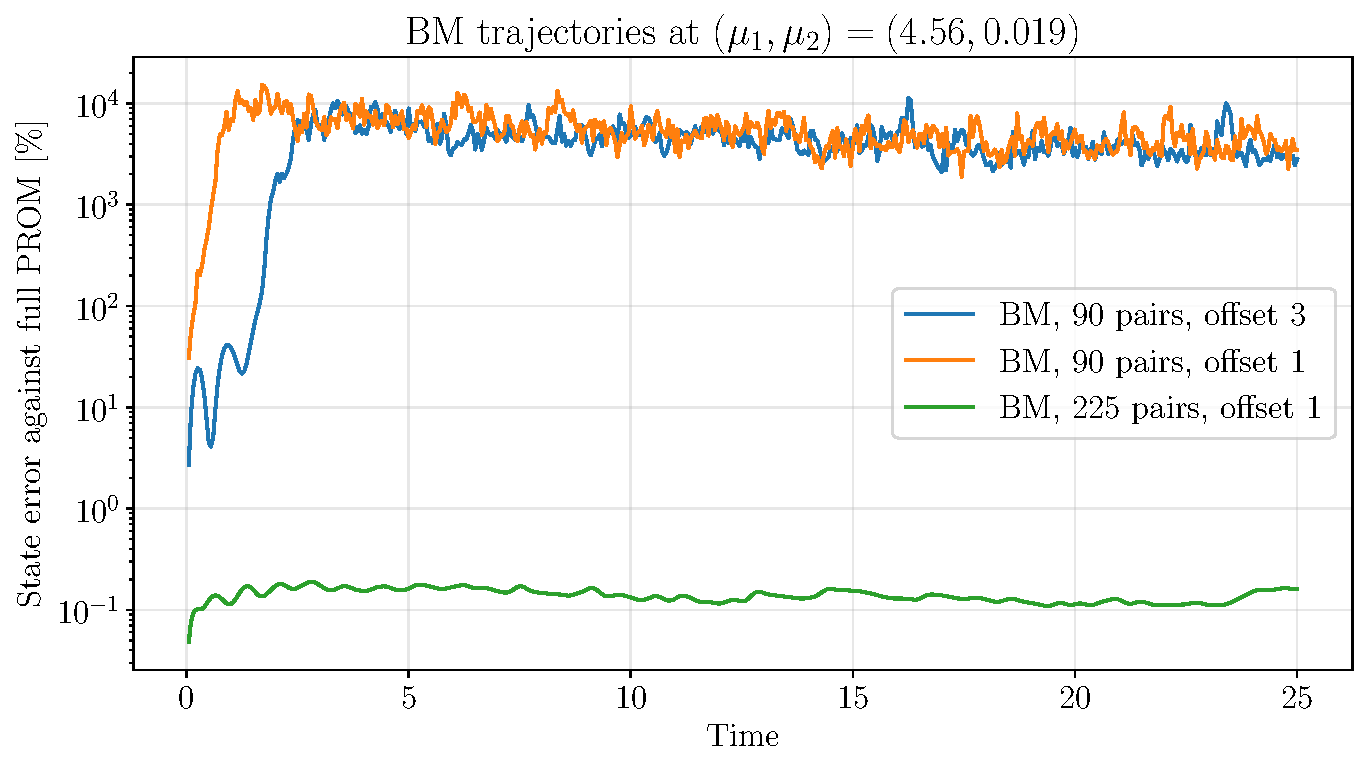
\includegraphics[width=0.96\linewidth]{figures/training_trajectory_diagnostic.pdf}
 \caption{Instantaneous BM trajectory errors against the full PROM at $\vect{\mu}=(4.56,0.019)$ for the 90- and 225-pair rules. These curves isolate comparison with the same trial-space model; they use a different reference from Table~\ref{tab:impl-accuracy}.}
 \label{fig:impl-diagnostic}
\end{figure}

These measurements support an explanation involving inaccurate updates and stronger local perturbation amplification in the insufficiently trained rules. They do not give a general instability proof: one sensitivity norm above one can occur even for the full PROM. Increasing the pair count also changes the selected cells and fitted weights, so we have not isolated pair count as the sole cause. Neither is 225 a demonstrated universal minimum. The failed and successful BM rules both allow nonsymmetric Jacobians, so loss of a common scalar potential alone does not explain why one works and another fails.

\subsection{Questions for discussion}
\label{sec:impl-questions}

\begin{enumerate}
 \item \textbf{What property should BM preserve in this setting?} Classical ECSW's structural result in Farhat, Chapman, and Avery~\cite{impl-farhat2015} relies on a weighted Lagrangian. Here the starting equations are finite-volume Burgers with forcing, inflow, and LSPG. We should specify the relevant discrete conservation or stability property before claiming that it is preserved locally or globally. For LSPG, common scalar weights retain a sampled residual objective, while mode-dependent weights do not generally retain one.
 \item \textbf{What should training control beyond contribution values?} The 90-pair fits show that a small training residual can coexist with poor updates outside the training pairs. Would additional states, Jacobian information, or time-update sensitivity improve robustness without requiring many more cells?
 \item \textbf{Is the signed candidate score the best shared-mesh selection rule?} We currently implement the proposal's signed sum. Comparing it with a score based on achievable error reduction could clarify the effect of cancellations between coordinates. Such a comparison has not yet been performed.
 \item \textbf{How much of the timing gain comes from the rule itself?} The current comparison matches training and reports every repeated run, but uses different nonlinear solvers and stopping quantities. A further comparison should control solver choices where the equations permit it and check accuracy and convergence alongside timing.
\end{enumerate}

The demonstrated result is narrower than these questions: on this 96-mode Burgers problem, a BM rule trained on 225 consecutive projected HDM pairs works at three unseen parameters with far fewer cells and shorter measured online times than our matched classical ECSW implementation.

\subsection{Files and reproduction}
\label{sec:impl-reproduction}

All paths below are relative to \texttt{burgers2d-rom-workbench}. The appended text is in \path{Project_BM-ECSW/BM_ECSW_LSPG_implementation.tex}; the original proposal and reading notes remain in \path{Project_BM-ECSW/ECSW_General_by_basis.tex}. The Burgers description and the HDM figure come from \path{Project_YvonMaday/Results_Paper/manuscript_paper_euclidean.tex} and its figure directory. That manuscript uses a different reduced dimension; all counts here refer to the current 96-mode experiment.

The implementation is in \path{run_hprom.py}, \path{burgers/linear_manifold.py}, and \path{burgers/gauss_newton.py}. The repeated measurements, individual reports, input hashes, and thread metadata are stored under
\begin{quote}\small
 \path{Results/ECSW_BM_benchmark_20261004T185223Z/}.
\end{quote}
The trajectory and sensitivity diagnostics are under \path{Results/BM_ECSW_diagnostics/}, generated by \path{diagnose_bm_ecsw.py}. The benchmark driver is \path{benchmark_ecsw_bm.py}. Its repeated timing command, from the repository root, is
\begin{quote}\small\ttfamily
 .venv/bin/python benchmark\_ecsw\_bm.py --repeats 3 --threads 20
\end{quote}
Tables and comparison figures are generated from the saved reports and weights by \path{Project_BM-ECSW/generate_results_figures.py}. They can be regenerated without retraining or rerunning online simulations:
\begin{quote}\small\ttfamily
 .venv/bin/python Project\_BM-ECSW/generate\_results\_figures.py
\end{quote}
Then compile \texttt{ECSW\_General\_by\_basis.tex} with \texttt{latexmk -pdf} inside \texttt{Project\_BM-ECSW}.

\begin{thebibliography}{9}
\bibitem{impl-barnett2023}
J.~Barnett, C.~Farhat, and Y.~Maday.
Neural-network-augmented projection-based model order reduction for mitigating the Kolmogorov barrier to reducibility.
\textit{Journal of Computational Physics}, 492:112420, 2023.

\bibitem{impl-carlberg2011}
K.~Carlberg, C.~Bou-Mosleh, and C.~Farhat.
Efficient non-linear model reduction via a least-squares Petrov--Galerkin projection and compressive tensor approximations.
\textit{International Journal for Numerical Methods in Engineering}, 86:155--181, 2011.

\bibitem{impl-grimberg2021}
S.~Grimberg, C.~Farhat, R.~Tezaur, and C.~Bou-Mosleh.
Mesh sampling and weighting for the hyperreduction of nonlinear Petrov--Galerkin reduced-order models with local reduced-order bases.
\textit{International Journal for Numerical Methods in Engineering}, 122:1846--1874, 2021.
DOI: \href{https://doi.org/10.1002/nme.6603}{10.1002/nme.6603}.

\bibitem{impl-farhat2015}
C.~Farhat, T.~Chapman, and P.~Avery.
Structure-preserving, stability, and accuracy properties of the energy-conserving sampling and weighting method for the hyper reduction of nonlinear finite element dynamic models.
\textit{International Journal for Numerical Methods in Engineering}, 102:1077--1110, 2015.
DOI: \href{https://doi.org/10.1002/nme.4820}{10.1002/nme.4820}.
\end{thebibliography}
\endgroup
